\label{sec:Intro}
There are many situations in which reference signals, or future disturbances are `previewable'. 
Optimal Preview Control is concerned with designing controllers that exploit previewed information in order to achieve performance levels that are superior to those achievable using current information alone. This paper considers the generic preview synthesis problem illustrated in Figure \ref{fig:DistRejSys}, which comprises a two-degree-of-freedom controller and both previewed disturbances/references ($r$), and unpreviewed disturbances ($w$).
An $\htwo$-optimal solution to this controller synthesis problem is provided that requires only low-dimensional computations and low-dimensional Riccati equation solutions, and leads to a controller whose high-dimensional component is a Finite Impulse Response (FIR) filter; the efficient implementation of FIR filters is well known is the signal processing literature.
The low-dimensional solution to the problem described in Figure~\ref{fig:DistRejSys} derives from the fact that the states of the (high-dimensional) delay line can be reconstructed by making a copy of $\Phi$ in the controller.  The objective of this paper is to provide a framework for synthesizing preview controllers for any problem that fits into the framework illustrated in Figure~\ref{fig:DistRejSys}.
\begin{figure}
\begin{center}
\stdcontrolfrags
\psfrag{Phi}{$\Phi$}
\psfrag{r}{$r$}
\psfrag{rhat}{$\hat r$}
\psfrag{eta}{$\eta$}
\psfrag{G_p}{$G_p$}
\includegraphics[height=4.0cm]{./diags/DistRejSys.eps}
\caption{\label{fig:DistRejSys} A generalized regulator problem with both previewable and non-previewable disturbances. The transfer function $G$ is the system to be controlled, $K$ is the controller to be synthesized and $\Phi$ is an $N$-step delay line. The disturbance $w$ is not previewable, the control and measurement signals are $u$ and $y$ respectively, $\hat r$ is the previewable disturbance, and $r$ is the future value of $\hat r$. The filter $W_r$ is used  model the expected frequency content of $r$.}
\end{center}
\end{figure}

One of the first papers to recognise the importance of preview control is \cite{Sheridan}; three preview control models are described. In the third of these models open-loop optimal preview controls are found using dynamic programming. The earliest applied work on preview control dates back to \cite{Bender_1968_PrevSusp}, where Wiener filter theory was used to design an active suspension with road preview. Bender's solution required the transfer function from the previewed path to the vehicle's acceleration to be unstable --- such a solution is not implementable. Much of the subsequent work on preview tracking has its origins in the 1973 PhD thesis of M. Tomizuka~\cite{Tomi_1973_Thesis}, in which  the preview control task is cast in a discrete-time linear quadratic regulator framework by augmenting the plant dynamics with a delay line model. In this formulation the number of states grows in direct proportion to the preview length and so a direct solution of the corresponding Riccati equations becomes computationally infeasible for long preview lengths. Tomizuka presented an efficient recursive method for solving these large equations. A continuous-time version of a LQ preview control problem is studied in \cite{Tomizuka_1975_ContinuousLQPreview}, while a continuous-time preview control problem is given a stochastic interpretation in \cite{Lindquist}.

In the context of the early literature, \cite{Tomizuka_1975_OptDiscretePreview} provides a good overview of an output-feedback preview-tracking problem with reference noise. This paper also summarizes many of the basic properties of preview feedback controllers. 
Motivated by a process control problem, another previewable command reference variant, the so-called proportional, integral, derivative, preview (PIDP) controller is studied in \cite{Tomizuka_1979_IntegralPreviewFI} in an LQ optimal control framework. A closely associated feedforward problem is studied in \cite{Tomi_1980_FFPrev}. Other schemes for computing a feedforward-only controller is given in \cite{Zattoni_2006_H2PreviewFF} and \cite{Marro_2005_FFH2Preview}. Bender's vehicle suspension preview problem is re-visited in \cite{Tomi_1976_SuspRevisited} in a discrete-time command preview framework. The preview suspension problem has attracted the attention of several practitioners in the more recent literature; examples include \cite{Hac_1992_Opt_Veh_Susp,Marzbanrad_2004_SuspPrev,Roh_1999_Stoc_Opt_Prev,Sharp_2005_CarHandlingPreview}.

We will use the problem formulation in Figure \ref{fig:DistRejSys} as a basis for the results presented here. A solution will be derived
by formulating the problem in a generalised regulator framework \cite{LimebeerGreen,ZDG}, and then finding efficient solutions to the resulting high-dimension Riccati equations. Contributions made by this paper include:
\begin{itemize}
\item An efficient method for finding the $\htwo$ norm of the closed-loop system;
\item a method for evaluating the benefit of preview;
\item a low-order output feedback controller implementation;
\item an analysis of the  generic properties of preview controllers.
\end{itemize}

Figure~\ref{fig:SimpleSISOPrev} illustrates a simple example that may be used to highlight the benefit of preview, the broad structure of the controller, and the effect of preview on the achievable $\htwo$-norm of the closed-loop system. 
\begin{figure}
\stdcontrolfrags
\begin{center}
\includegraphics[width=0.4\hsize]{./diags/SimpleExampleNominalNoK2.eps}
\end{center}
\caption{A simple SISO open-loop preview tracking problem. The transfer function $\Phi$ is an $N$-step delay, $G$ is the plant to be controlled, and $K$ is the feedforward controller.}
\label{fig:SimpleSISOPrev}
\end{figure}

Assume that $G$ is stable. In the case when $G(\z)$ has all its zeros inside the unit circle, perfect tracking may be achieved by simply setting $K(\z)=G(\z)^{-1}\Phi(\z)$. 
However, if $G(\z)$ is non-minimum phase (NMP), then such a $K(\z)$ is not internally stabilising and a controller must be found that recognises the limits imposed by NMP zeros on the achievable tracking performance. Such limitations are well known for non-preview systems (i.e. $N=0$ and $\Phi=I$), and are investigated in some detail in \cite{Middleteon_2004_PrevPerf} and \cite{Mirkin_2004_FixedLagPerfSaturation} for the preview case.

It is clear from Figure~\ref{fig:SimpleSISOPrev} that the error system is given by $E(\z)=G(\z)K(\z)-\Phi(\z)$. If $G(\z)$ has an inner-outer factorization \cite{LimebeerGreen,ZDG} $G(\z)= G_o(\z) G_i(\z)$, we can write $E(\z)= (\tilde{K}(\z) -\Phi(\z)G_i(\z^{-1}))G_i(\z)$ in which $\tilde{K}(\z)= K(\z) G_o(\z)$ and
$G_i(\z^{-1})G_i(\z)=1)$. The optimal controller is found by setting $K(\z) = (\Phi(\z)G_i(\z^{-1}))_+ G_o^{-1}(\z) $, in which $(\cdot)_+$ denotes the stable projection \cite{LimebeerGreen,ZDG}. In the specific example of 
\als{
G(\z)&=\frac{\z-c_z}{1-\z c_z}G_o(\z) & &\szo{c_z}{},|c_z|>1,
}
it follows by direct calculation that
\als{K(\z)&=\underbrace{G_o(\z)^{-1}}_{IIR}\underbrace{\left(-c_z^{-1}\z^{-N} +  (1-c_z^{-2})c_z \sum^N_{i=1}(\z^{i-N}/c_z^i) \right)}_{FIR},
\intertext{and that}
\nrm{E(\z)}_2&=\frac{1}{\left|c_z^{N+1}\right|}\sqrt{c_z^2-1}.}
%
Since $\nrm{E(\z)}_2\rightarrow 0$ as $N\rightarrow \infty$, one concludes that in this example preview action can overcome completely the tracking limitation
imposed by the NMP zero. It is also clear that the controller contains a high-order finite impulse reponse (FIR) part and a low-order infinite implulse response (IIR) part; the preview action comes from the FIR part. The dynamics of the FIR block are fully specified by the RHP zero, $c_z$, and the preview length, $N$.

A pole-zero plot of the optimal controller is given in Figure \ref{fig:PZforSISOPrevH2} for the case where $c_z=1.05$, $G_o(\z)=(1-\z c_z)/(\z-0.5)$, and $N=20$. Notice the almost pole-zero cancellation on the real axis. In the limit $N\rightarrow \infty$ cancellation occurs. 
\begin{figure}
\begin{center}
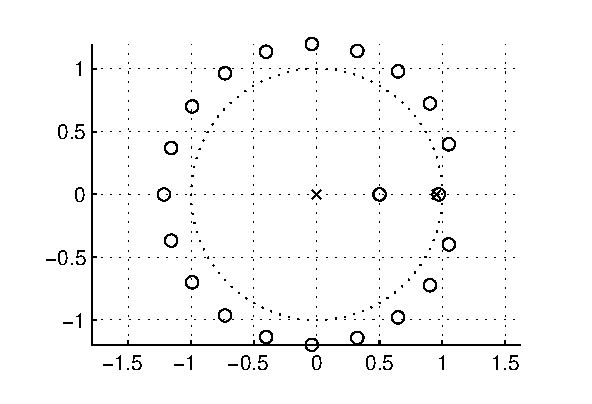
\includegraphics[width=0.7\columnwidth]{./diags/SimpleExamplePZPlot2.eps}
\end{center}
\caption{Pole-zero plot of the $\htwo$-optimal $K(\z)$ for the case where $c_z=1.05$, $G_o(\z)=(1-\z c_z)/(z-0.5)$ and $N=20$.   }
\label{fig:PZforSISOPrevH2}
\end{figure}

An obvious conclusion to be drawn from this example is that preview is potentially useful when designing feedforward controllers for NMP systems. If one has a control problem with an unstable plant, which is stabilised by a feedback controller, then the resulting closed-loop will often be NMP, and so preview action is also potentially useful when controlling unstable systems.

The paper is structured as follows: Preliminaries and some standard notation is given in Section~\ref{sec:notation}. A state-space description of the generalized regulator problem with both previewable and non-previewed exogenous disturbances is derived in Section~\ref{sec:Sys}. The solution of this problem, which is illustrated in Figure~\ref{fig:DistRejSys}, is the central focus of the paper. Following a summary of the general theory, the full-information preview control problem is solved in Section~\ref{sec:H2FI}. The results are mainly concerned with efficient algorithms for solving the $\htwo$ full-information Riccati equation, and the evaluation of the full-information feedback gain matrix. The solution of the output feedback preview problem is given in Section~\ref{sec:H2OF}. The output feedback controller involves a combination of a state-estimator, and the solution to the full-information problem. An efficient controller synthesis is also given in this section. The effect of preview in reducing the $\htwo$-norm of the closed-loop system is analysed in Section~\ref{sec:2norm}. The special case of feedforward control with preview is analysed in Section~\ref{sec:Preproc}. A summary of the main features of preview controllers, as well as some design insights, are given in Section~\ref{sec:H2PrevSum}. The conclusions are given in Section~\ref{sec:Conclusions}.